\subsection{Test Setup}

We benchmark \textsl{LazyBoE} against a number of kinodynamic planners with forward propagation, namely RRT \cite{lavalle2001randomized}, SST \cite{li2016asymptotically}, and BoE \cite{shome2021asymptotically}.\footnote{Links to our code, videos, and demonstrations of the experiments are available here: \href{https://hiro-group.ronc.one/research/lazyboe-icra24.html}{https://hiro-group.ronc.one/research/lazyboe-icra24.html}.} We test three variants of SST based on different selection-to-pruning radius ($0.5$x, $1$x, and $2$x).
Each algorithm is evaluated over $25$ planning problems, i.e., pairs of collision-free, randomly-sampled start and goal joint angles, on four metrics: i) \textsl{time to initial solution} in seconds (\cref{fig:eval-time}), ii) \textsl{final solution cost} as measured by the arclength of the trajectory in joint angle space (\cref{fig:eval-cost}), iii) \textsl{success rate} denoted by the fraction of trials that resulted in at least one planned trajectory (\cref{fig:eval-success}), and iv) \textsl{number of solutions} per planning problem (\cref{fig:eval-num_solutions}). 
This delineation into time to initial solution and final solution cost is necessitated by the fact that SST, BoE, and \textsl{LazyBoE} are asymptotically optimal in nature. All algorithms were implemented in Python 3.8 and evaluated on a 6-core AMD Ryzen 5 laptop with 32GB RAM running Ubuntu 20.04. Each algorithm was given a time budget of $60$s, except RRT, which terminates on the first solution.
\begin{figure}\label{fig:eval-time}
  \centering
    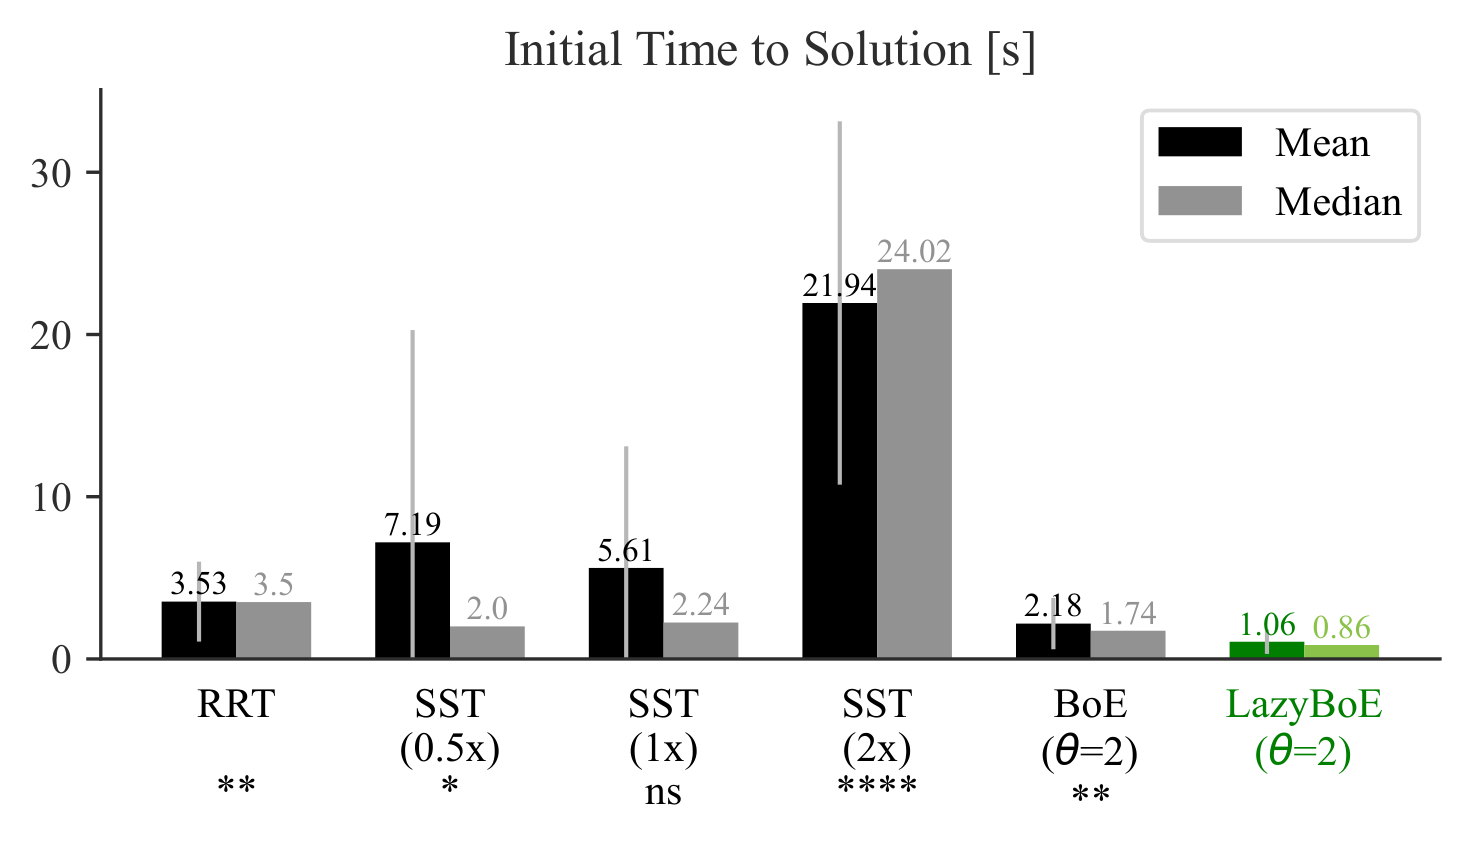
\includegraphics[width=\columnwidth]{assets/initial_planning_time.png}
  \caption{Our method is able to find the first solution in less time than baseline approaches, owing to its lazy approach to simulation and collision checking. Asterisks indicate significance level when comparing our planner to the baseline methods. \textsl{ns} indicates no significant difference.}\label{fig:eval-time}
\end{figure}
